\documentclass[a4paper, 11pt]{article}

\voffset -0cm
\hoffset 0.0cm
\textheight 23cm
\textwidth 16cm
\topmargin 0.0cm
\oddsidemargin 0.0cm
\evensidemargin 0.0cm

\usepackage{epsfig}
\usepackage{setspace}
\usepackage{fancyheadings}
\usepackage{amsmath}
\usepackage{amssymb}
\usepackage{graphicx}
\usepackage{url}

\title{}
\author{}
\date{}

\begin{document}

\begin{center}
	\LARGE \textbf{TP7: Curvature estimation of digital curves}
\end{center}

\begin{figure}
  \centering
  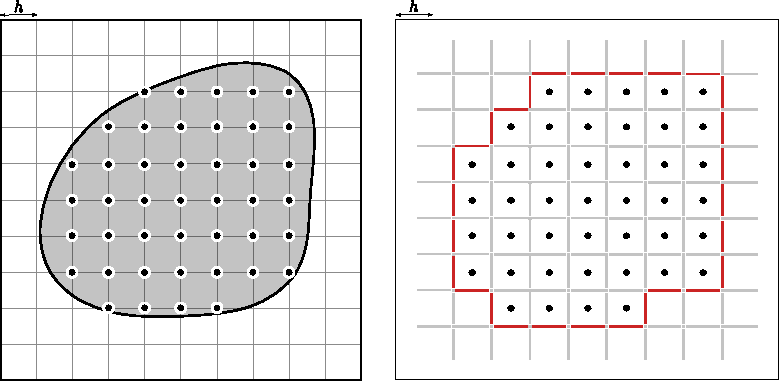
\includegraphics[width=0.8\textwidth]{gauss}
  \caption{The Gauss Digitization $\mathtt{D}_h(X)$ of and Euclidean shape $X$ (in gray) is the set of black points that lies within $X$.
  The set of surfels of the Gauss Digitization is pictured in red. }
  \label{fig:gauss}
\end{figure}

\begin{figure}
  \centering
  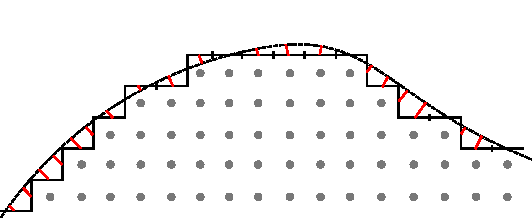
\includegraphics[width=0.8\textwidth]{proj}
  \caption{For a given linel $l$, the projection map $\xi$ associates the centroid of $l$ to the closest point on $X$.}
  \label{fig:proj}
\end{figure}

We consider a compact shape $X \in \mathbb{R}^2$. The Gauss Digitization of $X$, namely $\mathtt{D}_h(X)$, at a grid step $h$ is:
\[
  \mathtt{D}_h(X) := X \cap (h\mathbb{Z})^{2},
\]
which is simply the set of points of the infinite regular grid of size $h$ that are inside $X$ (see Fig.\ref{fig:gauss}).
The discrete border of $\mathtt{D}_h(X)$ is roughly defined as the border of the shifted $h + h / 2$-grid. In 2D, elements of dimensions $1$ are called linels
and elements of dimension $0$ are called pointels (they correspond to the center of the original $h$-grid). The set of linels is denoted $\mathbb{E}^1$ and the set
of pointels $\mathbb{E}^0$ for convenience.

For each elements of $l \in \mathbb{E}^1$ we call the projection of $l$ the closest point of the centroid of $l$ on $X$ (see Fig.\ref{fig:proj}). The associated
map is denoted $\xi$ and is called the projection map between $X$ and $\mathtt{D}_h(X)$.

\paragraph{Goal} Compute a convergent estimator $\tilde{\kappa}$ of the real curvature $\kappa$ at a point $x \in X$ using only the discrete structure. More precisely we want that $\forall \bf{x} \in \mathbb{E}^1$
\[
  || \kappa( \xi( \dot{\bf{x}} ) ) - \tilde{\kappa}( \dot{\bf{x}} ) ||_\infty \leq \sigma( h )
\]
where the limit of $\sigma$ is zero as $h$ tends to zero.

\section*{Integral Invariant Estimator}

\begin{figure}
  \centering
  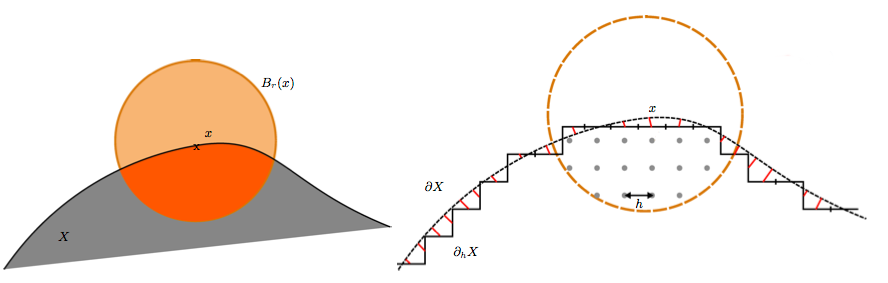
\includegraphics[width=\textwidth]{integral}
  \caption{The volumetric integral (on the left) $V_R(x)$ is the area of the intersection between an euclidean ball $B_r(x)$ centered in $x$ and the shape $X$.}
  \label{fig:integral}
\end{figure}

Given an euclidean ball $B_r(x)$ of radius $r$ centered in $x$, we define the volumetric integral $V_r(x)$ (see Fig.\ref{fig:integral}) as
\[
  V_r(x) := \int_{B_r(x)} \mathcal{X}(p)dp
\]
where $\mathcal{X}$ is the characteristic function of $X$ (it is equal to one if $x$ is in $X$, zero otherwise).

We have
\[
  \kappa(x) \approx \frac{3 \pi}{2r} - \frac{3 V_r(x)}{r^3}
\]
that links the curvature $\kappa$ and the volumetric integral $V_r$ at a point $x$. If we are able to compute the volumetric integral at a point $x$,
we can estimate the curvature at the same point.

An existing result for digital area approximation is
\[
  \text{Area}( \mathtt{D}_h(X) ) := h^2 \text{Card}(\mathtt{D}_h(X)) = \text{Area}(X) + O(h)
\]
where $\text{Card}$ is simply the number of digital points within $\mathtt{D}_h(X)$. Therefore, to estimate $V_r(x)$ we can count the number of digital points in the intersection
between $B_r(x)$ and $\mathtt{D}_h(X)$.

In order to achieve convergence of the estimator $\tilde{\kappa}$, the ball radius $r$ must be set to $k h^{\frac{1}{3}}$ where $k$ depends on the shape.

\section*{Assignment}

You have to implement the integral invariant curvature estimator $\tilde{\kappa}$ on 2D digital curves. To do so, have a look at the file generate\_digital\_contour.cpp in DGtalSkel.
This program computes the Gauss Digitization $\mathtt{D}_h(X)$ (where $X$ can be here either a Ball, a Flower or and Accelerated Flower), extracts its digital border
and finally gives the real curvature by projecting digital points onto $X$.

\paragraph{Question} Given a surfel $\bf{s}$, implement the estimator of the volumetric integral (it must be parametrized by the ball radius $r$)

\paragraph{Question} Implement the curvature estimator $\tilde{\kappa}$. For each linels $l$, compute the mean of the volumetric integral estimator of the two adjacent surfels.

\paragraph{Question} Plot (using gnuplot for example) the maximum error between the real curvature $\kappa$ and the estimated one $\tilde{\kappa}$ with a decreasing grid-step $h$.

\end{document}
